
\documentclass[runningheads]{llncs}

\usepackage{graphicx}
\usepackage{float}
\usepackage{algorithm}
\usepackage[noend]{algpseudocode}

\begin{document}
%
\title{Ordonnancement multicast pour optimiser la consommation d'énergie avec des contraintes de temps}
%
\titlerunning{Ordonnancement multicast \dots}

\author{Isma\"il Bagayoko\orcidID{BAGI14069802}}
%
\authorrunning{I. Bagayoko}

\institute{Universit\'e du Qu\'ebec \`a Montr\'eal \\
\email{bagayoko.ismail@courrier.uqam.ca}\\
\url{} }
%
\maketitle              % typeset the header of the contribution
%
\begin{abstract}
Ces dernières années, le trafic mobile a considérablement augmenté. 
Il y a une similitude dans les demandes de données au niveau station 
de base. Les requêtes pour les mêmes données sont à des intervalles 
de juste quelques microsecondes, la station de base se trouve à faire des 
opérations très répétitives. 

L'ancienne méthode où les requêtes sont servis une à la fois ne 
fonctionne plus, il n'est pas rentable en matière de ressources 
(ex: énergie). C'est là qu'intervient la multi-diffusion (multicast), 
elle consiste à servir plusieurs requêtes en un seul envoi (réponse).
Il faut attendre de recevoir  plusieurs requêtes pour les servir en 
un seul envoi. On s'aperçoit tout de suite que l'idéal c'est d'attendre 
infiniment et servir. Les premières requêtes vont donc beaucoup attendre pour 
être servis.

Nous présentons trois approches pour ordonnancer les requêtes, afin de 
réduire la consommation des ressources et le délai.

% Il y a un compromis à  faire ici, plus on attend plus on économise en 
% ressources mais plus l'on attend plus nous perdons en matière de qualité 
% de service. Un exemple d'utilisation est un fournisseur d'accès internet 
% qui veut minimiser l'utilisation des ressources mais respecter les d\'elais 
% payés par les clients.

La multi-diffusion bien qu'existe depuis longtemps, au cours des 
dernières années elle a suscité beaucoup d'intérêt dû aux nombreux 
avantages qu'elle apporte: le coût en énergie, l'utilisation efficace 
du canal et bien d'autres.


\keywords{Multicast \and Algorithme g\'en\'etique  \and Algorithme glouton. }
\end{abstract}
%
%
%
\section{Introduction}
% Motivation
Avec l’essor des smartphones et objets connectés en réseau, la demande en données 
est massive et croissante. La cinquième génération (5G) de systèmes de 
communication sans fil est la réponse pour satisfaire ces nouvelles exigences.
Pour répondre aux nouvelles exigences, de nouvelles technologies doivent 
être introduites. D’autres technologies, qui autre fois non réalisable en 
raison de la puissance de calcul, doivent êtres revisité (multi-diffusion).

% Problématique
La multidiffusion permet de servir  plusieurs utilisateurs  le même contenu dans 
la même transmission. L'ancienne méthode (mono-diffusion) où les requêtes sont servis 
une à la fois ne fonctionne plus, elle n'est pas rentable en matière de 
ressources (ex: énergie). C'est là qu'intervient la multi-diffusion (multicast).
Il faut attendre de recevoir  plusieurs requêtes pour les servir en un seul
envoi. On s'aperçoit tout de suite que l'idéal c'est d'attendre le plus longtemps
possible puis servir. Les premières requêtes vont beaucoup attendre pour 
être servis.
% Nous servons plusieurs utilisateurs en une seule séance tout en respectant le délai.

% État de l'art
L'ordonnancement multidiffusion a reçu toute l'attention au cours des 
dernières années en raison de sa capacité à réduire l'utilisation 
des ressources dans la communication cellulaire.

Les auteurs de \cite{inho2015} présentent un schéma bas\'e sur l'état 
des canaux basé sur la qualité pour une planification gloutonne de multidiffusions.

Les auteurs de \cite{inho2017} et \cite{hang2017} proposent un 
compromis entre l'utilisation des ressources et l'équité en introduisant 
de multiple  seuils condition de canal par groupe.


% Organisation
Le reste de ce projet est organis\'e comme suit: D'abord, nous 
présenterons le modèle de réseau, suivit de la formulation du 
problème d'ordonnancement. Enfin, nous fournirons des résultats 
numériques. 



\section{Modèle de système}
On considère un système avec une station de base (BS), ayant en mémoire 
un certain nombre de contenus (message m) fréquemment demandés, avec comme 
moyen de transmission utilisé est un système de transmission multicast.

Tous les messages disponibles au niveau de la station de base sont associés 
à un groupe constitué de stations mobiles (MS) demandant le message pendant 
un slot de temps.
On considère alors que la taille de chaque message est d'une unité et qu'il 
faut une unité de temps pour le transmettre.

Nous utilisons une pénalité de retard, uniformément répartie et 
$ d_i  $ est le d\'elai associé \`a la requête  $ i $. Si la requ\^ete 
n'est pas r\'epondu dans le délai la p\'enalit\'e de retard est appliqu\'ee.

Notre ordonnanceur multicast doit prendre la décision d'envoyer ou non 
un message pendant un créneau horaire, afin de minimiser la consommation 
d'énergie sur le long terme tout en respectant un délai raisonnable sur toutes les demandes.

Chaque requête est définit par quatre composants:
\begin{itemize}
    \item $a_i$ est l'instant d'arriver de la requête $i$
    \item $d_i$ est le dernier instant que peut tolérer la requête $i$
    \item $m_i$ est l'identifiant du contenu (message) demandé par la requête  $i$
    \item $e_i$ l'énergie nécessaire pour répondre à la requête $i$
\end{itemize} 

L'énergie pour un groupe émetteur à $ t $ est la même que l'énergie de la 
requête qui a la mauvaise condition de canal (Plus grande énergie) à $ t $.
La consommation d'énergie est définie comme dans \cite{huang2016}:
\begin{equation}
    E_r(t)  =  \frac {C} {| h ^ 2 |}  
\end{equation}
o\`u $C$ est la capacité  de notre station de base et $h$ l'état du canal.

\begin{figure}[H]
    \centering
    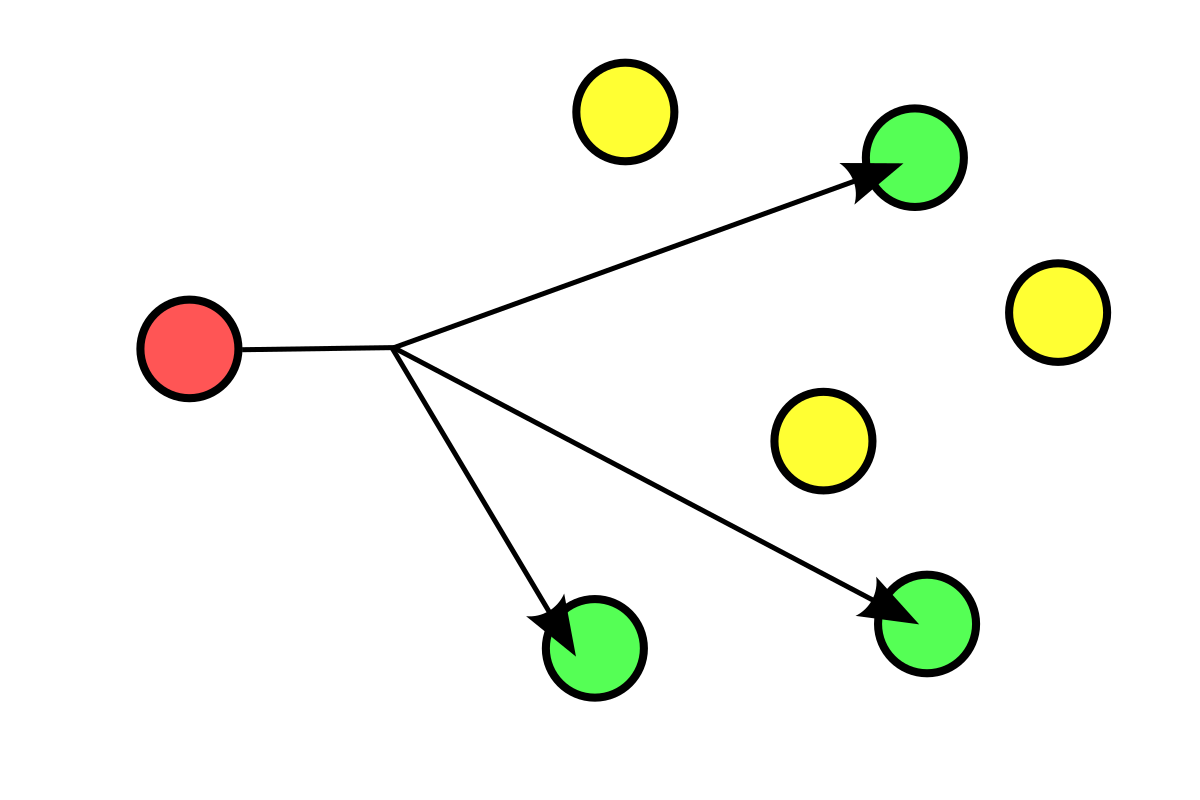
\includegraphics[scale=0.2]{multicast.png}
    \caption{Source: Wikipedia
    \url{https://en.wikipedia.org/wiki/Multicast}
    [visité en avril, 2020]}
\end{figure}
\section{Formulation du problème}
Nous considérons un ensemble $R$ de requêtes défini comme 
$R = \{(a, d, m, e )_i\} $ 


On définit les variables de décision:
\begin{itemize}
    \item $x_i$ est l'instant d'envoi de la requête $i$ à  déterminer 
    \item $y_m$ est l'instant d'envoi du message  $m$ à  déterminer 
    \item $E_t$ représente l'énergie consommée a un instant $t$
    \item $E_t^m$ représente l'énergie consommée a un instant $t$ pour 
    le message $m$
\end{itemize}

Nous consid\'erons les deux cas suivant lorsqu'un seul contenu o\`u plusieurs 
sont disponibles pour la multidiffusion est disponible au niveau de la 
station de base.

\subsubsection{Pour un message} la decision d'ordonnancement est simple, il 
consiste a répondre a une seul question: Quand transmettre ?
\[
    \begin{array}{cc}
         \textbf{minimiser} &  \sum\limits_{t} E_t\\
         \textbf{Sous contraintes} & \\
         & E_t = \max\limits_{x_i=t} e_i \\
         & a_i \leq x_i \leq d_i\\
    \end{array}
\] 

\subsubsection{Plus d'n message}
On a plusieurs questions cette fois-ci :
Quel message doit être transmis?  Quand le transmettre ?
Il faut ajouter une condition pour que deux messages différents ne puissent pas être 
envoy\'es au même moment.

L'idée c'est de dire qu'un seul $E_t^m$ peut être différent de zéro a la fois.
\[
    \begin{array}{cc}
         \textbf{minimiser} &  \sum \limits_{m}\sum\limits_{t} E_t^m\\
         \textbf{Sous contraintes} & \\
         & a_i \leq x_i \leq d_i\\
         & E_t^m = \max\limits_{x_i=t \textbf{ et } m_i=m} e_i \\
         & \sum\limits_{m}  1_{ E_t^m\geq 0} \leq 1 \textbf{ pour l'ensemble des messages} \\
    \end{array}
\]

\section{Solutions propos\'es }
Nous présentons trois approches pour ordonnancer les requêtes, afin de 
réduire la consommation ressources et le délai.

\subsection{Une approches na\"ive }
Elle consiste à vérifier toutes les solutions possibles et d'en choisir une(la meilleure).
Avec l'ensemble des requêtes, nous générons tous les regroupements possibles.
Ceci est équivalent à générer toutes les partitions d'un ensemble.
le nombre de partition d'un ensemble $S$ est $2^{|S|}$.
Le pseudo-code suivant représente les principales étapes de l'algorithme.
\begin{algorithm}[H]
    \caption{Na\"ive}%
    \label{alg:naive}
    \begin{algorithmic}[1]
        \State {$P \gets $ Toutes les partitions de $R$}
        \For{$p \in P$}
        \Comment{Pour chaque partition}
        \State{Verifier si la partition respecte les contrainte}
        \State{Calculer la consommaion d'energie et le delai}
        \EndFor{}
        
        \State{Choisir la partition qui consomme le moins d'\'energie}
    
        % return energie[i], delay[i]
    \end{algorithmic}
\end{algorithm}


  
\subsection{Une m\'ethode gloutonne}
Pour l'algorithme glouton la prise de décisions  est locale. 
Il n'ordonnance pas avec anticipation des répercussions d'une décision.

Notre algorithme glouton récupère la requête qui coûte le plus en transmission.
À cette requête il essaie d'ajouter toutes les requêtes qu'il peut en respectant 
les différentes contraintes. 
l'algorithme fait cela jusqu'à ce qu'il n'y ait plus de requête à laquelle répondre.
\emph{La demande sélectionnée ayant la plus grande consommation d'énergie, 
la consommation du groupe sera la même.}

Nous observons une complexité  de $O(|R|^2)$
\begin{algorithm}[H]
    \caption{Glouton}%
    \label{alg:greedy}
    \begin{algorithmic}[1]
      \While{$R \ne \emptyset$}
        \State{$ G \gets \emptyset $}
        \State{$ S \gets$ requ\^ete qui demande la plus grande \'energie }
        \State $ R \gets R - \{S\}$
        \State $ G \gets G \cup \{S\}$
      % $remove(no\_scheduled, selected)$\;
      % $add(multicast\_group, selected)$\;
      
      \For{$r \in R$} 
           \If{$r$ peut être ajouté à $G$}
            \State{ $ R \gets R - \{r\}$}
            \State{ $ G \gets G \cup \{r\}$}
          \EndIf{}
       \EndFor{}
       Planifier $G$ pour temps de $S$
      \EndWhile{}
    \end{algorithmic}
  \end{algorithm}

\subsection{Un algorithme g\'en\'etique}
Pour mettre en place l'approche génétique nous avons plusieurs prérequis:
\subsubsection{Un individu de la population :} 
Comment représenter un individu de la population?
Nous utilisons un système d'indices (ou intervalles) pour représenter une partition. 
Un individu est une représentation d'une partition.

\paragraph{Exemple : } Soit l'ensemble $\{1, 2, 3, 4\}$ 
Les indices de partitions possibles sont :
$[[0, \textbf{Fin}], [0,1, \textbf{Fin}], [0,1, 2, \textbf{Fin}], [0,1, 2, 3, \textbf{Fin}], [0,1, 3, \textbf{Fin}], [0,2, \textbf{Fin}], [0,2, 3, \textbf{Fin}], [0,3, \textbf{Fin}]]$

L'individu [0, 1, 2, \textbf{Fin}] permets de générer la partition :  $\{\{0\}, \{1\}, \{2, 3\}\}$
\begin{itemize}
    \item de l'indice $0$ \`a $1$ forme un sous ensemble : $\{0\}$
    \item de l'indice $1$ \`a $2$ forme un sous ensemble : $\{1\}$
    \item de l'indice $2$ \`a \textbf{Fin} forme un sous ensemble : $\{3, 4\}$
\end{itemize}
\begin{table}[H]
\centering
\caption{D'autres examples de partition de indices}\label{tab1}
\begin{tabular}{|l|l|}
\hline
Indices (Individu) &  Partition \\
\hline
$[0, \textbf{Fin}]$&  $\{\{0, 1, 2, 3\}\}$\\
$[0,1, 2, 3, \textbf{Fin}]$ & $\{\{0\}, \{1\}, \{2\}, \{3\}\}$\\
$[0,1, \textbf{Fin}]$ & \{\{0\}, \{1, 2, 3\}\}\\
\hline
\end{tabular}
\end{table}

\subsubsection{Le passage à la nouvelle génération:}
Ici nous avons considéré que la mutation comme moyen 
d'\'evolution de la population. En le principe un sous-ensemble de la partition 
est choisit afin d'\^etre agrandit ou  réduit.

Les répercussions que peut avoir cette operation est la fusion de 
deux sous ensemble ou la division d'un sous ensemble en deux.

\begin{algorithm}[H]
    \caption{Génétique}%
    \label{alg:genetic}
    \begin{algorithmic}[1]
        \State {$P \gets $ générer une population}
        \State {$S \gets$ meilleur individu de notre population $P$}
        \While{$i <$ Nombre maximum d'iterations }
            \For{Individu dans $P$}
                \State Fils $ \gets  $\Call{NouvelleGeneration}{Individu}
                \State Individu $\gets $ Fils
                \If{Fils.Energie < S.score}
                    \State{ $S \gets $ Fils}
                \EndIf{}
            \EndFor{}
        \EndWhile{}

    \State \Return{$S$}
    
        % return energie[i], delay[i]
    \end{algorithmic}
\end{algorithm}
\begin{algorithm}[H]
    \caption{NouvelleGeneration}%
    \label{alg:ngeneration}
    \begin{algorithmic}[1]
        \State{sélectionner au hasard un sous-ensemble}
        \State{Fils1 $\gets$ le sous-ensemble agrendit}
        \State{Fils2 $\gets$ le sous-ensemble r\'eduit}
        \State{Fils3 $\gets$ augment\'e le nombre de sous ensemble}
        \State{Calculer les scores}
    \State \Return{Le fils avec le meilleur score}
    
        % return energie[i], delay[i]
    \end{algorithmic}
\end{algorithm}



\section{R\'esultats num\'eriques}
Pour évaluer les performances de nos algorithmes, nous avons estimé la 
consommation totale d'énergie en fonction du trafic au niveau de notre station de 
base dans un premier temps. Le délai des utilisateurs est aussi mesur\'e.
Dans notre simulation, nous considérons que le gain du canal est constant 
et suit une distribution uniforme de \cite{huang2016}.
Nous considérons également les valeurs d'initialisation de \cite{huang2016} 
pour le bruit $ \tau $ comme une unité et la puissance $ \rho $ comme 
$ 1 watt $. Pour le débit de données, nous utilisons $1Kb/ms/1Mhz$.
La simulation est faite sur une durée de T =20. 
Le délai $d$ d'une requête est généré entre [1, 5].



\subsection{Consommation d'\'energie vs Charge du syst\`eme}
Fig.~\ref{fig:evslm1} et ~\ref{fig:evslm4}  repr\'esentent la consommation d'énergie sur 
la charge du système (nombre de requêtes par unit\'e de temps) avec 1 et 4 messages.
Au tout début, nos méthodes ont des consommations similaire parce que les
trois font de la mono diffusion (unicast). Le nombre de requêtes n'est pas 
assez nombreux pour du multicast.
L'algorithme g\'en\'etique n'est pas stable, ceci est dû au caract\`ere 
aléatoire dans sa pratique.
\begin{figure}[H]
    
    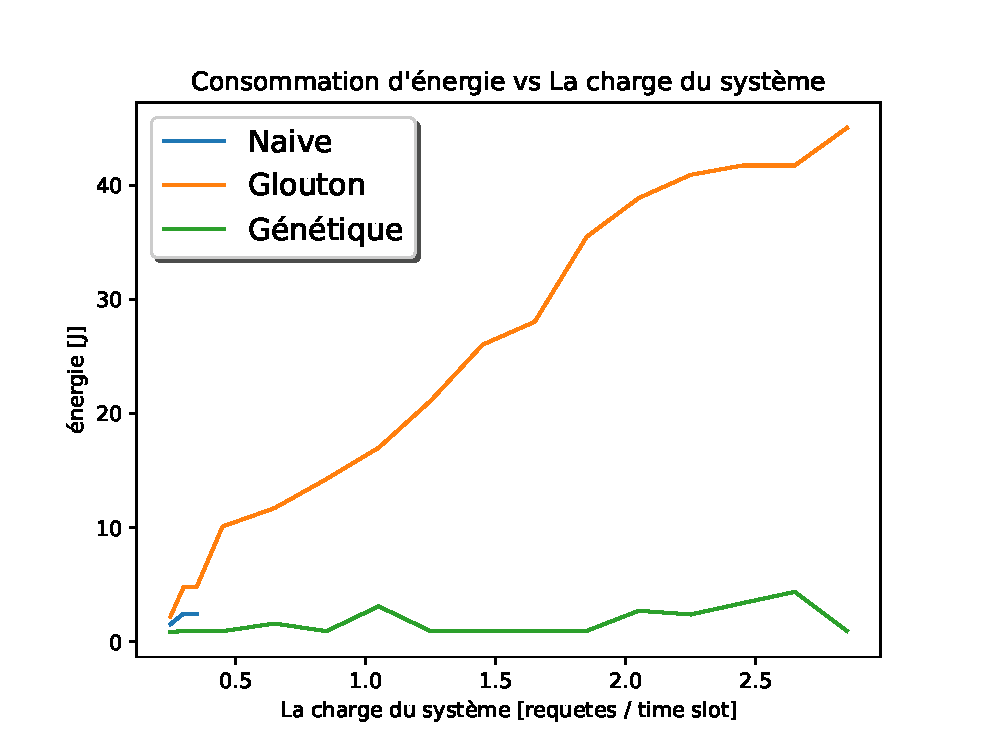
\includegraphics[width=\textwidth]{EvsL1.eps}
    \caption{Consommation d'énergie vs La charge du système, pour 
    le nombre de contenu disponible \`a la station de base $m=1$} 
    \label{fig:evslm1}
\end{figure}

\begin{figure}[H]
    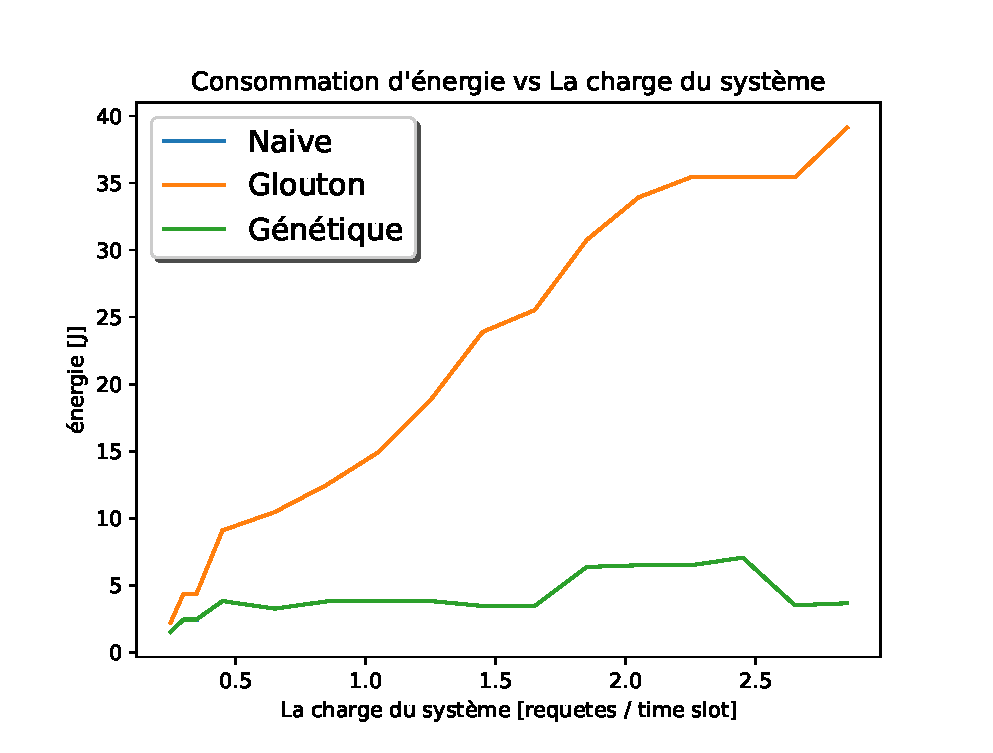
\includegraphics[width=\textwidth]{EvsL4.eps}
    \caption{Consommation d'énergie vs La charge du système, pour 
    le nombre de contenu disponible \`a la station de base $m=4$} 
    \label{fig:evslm4}
\end{figure}

Nous avons utilisé une différente fonction pour évaluer la consommation 
d'énergie pour l'algorithme génétique.
La contrainte qui dit qu'un seul message doit être envoyé à la 
fois n'est  pas respecté a chaque fois.
On accepte cette exception mais avec des pénalités. 
on peut observer les compromis sur Fig.~\ref{fig:dvslm1} et \ref{fig:dvslm4}
\subsection{Pénalité délai vs Charge du syst\`eme}
Sur les fig.~\ref{fig:dvslm1} et \ref{fig:dvslm4} on peut observer les pénalités 
de retard pour la solution génétique. 
Ce qui offre une qualité de service assez mauvaise aux utilisateurs. Même si le 
coût d'opération est peu coûteux
l'algorithme glouton réduit la consommation des ressource avec toujours le délai satisfait.
La satisfaction du délai est incontournable
\begin{figure}[H]
    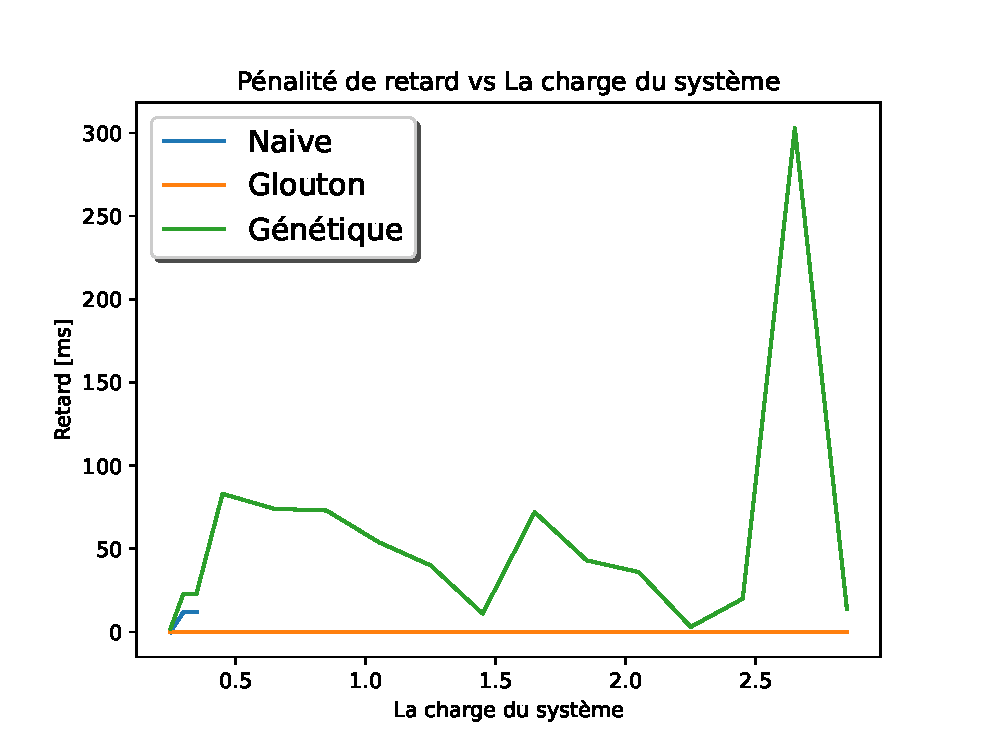
\includegraphics[width=\textwidth]{DvsL1.eps}
    \caption{Pénalité de retard vs La charge du système, pour 
    le nombre de contenu disponible \`a la station de base $m=1$ } 
    \label{fig:dvslm1}
\end{figure}
\begin{figure}[H]
    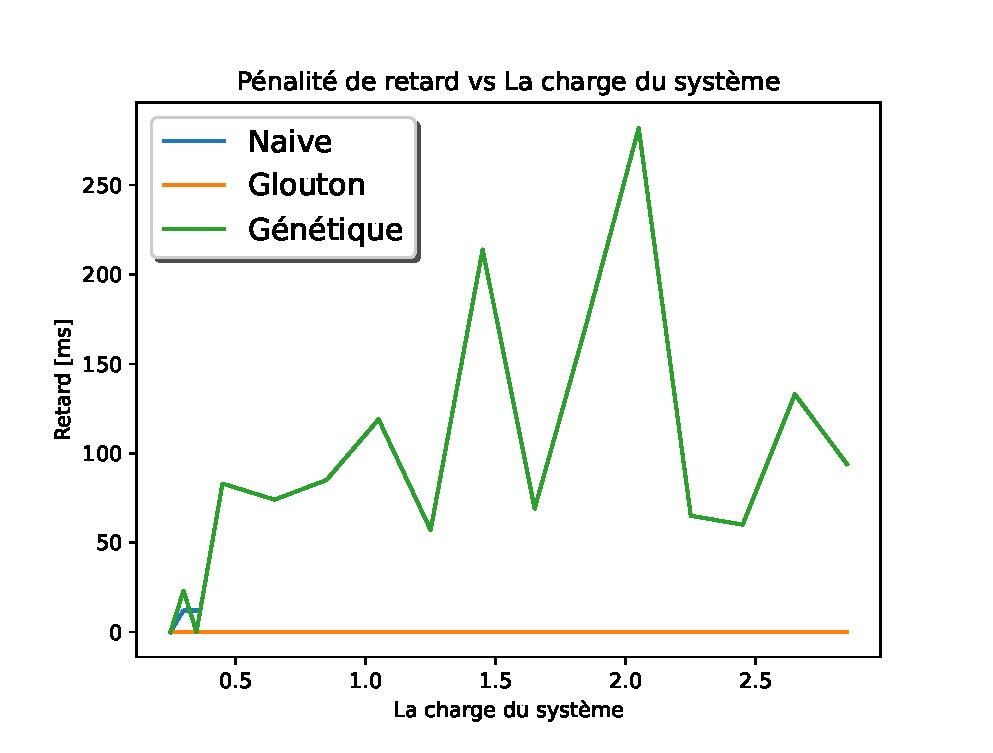
\includegraphics[width=\textwidth]{DvsL4.eps}
    \caption{Pénalité de retard vs La charge du système, pour 
    le nombre de contenu disponible \`a la station de base $m=4$ } 
    \label{fig:dvslm4}
\end{figure}

% \subsection{Consommation d'\'nergievs Maximum de delai}


% \subsection{Temps d'ex\'ecution vs Charge du syst\`eme}


\section*{Conclusion}
Après avoir proposé une solution naïve nous avons présent\'e deux 
solutions de faible complexités 
pour l'ordonnancement de multicast de plusieurs messages.
Les deux solutions ont chacune leur point forts.
L'algorithme glouton respecte toujours le délai même si 
la consommation des ressources n'est pas la meilleure.

L'algorithme génétique réduit à consommation des ressources 
mais les utilisateurs doivent attendre pour recevoir leurs données.

Nous avons présent\'e également des résultats numériques pour la 
consommation d'énergie de la station de base dans différents scénarios.
Ils montrent comment la station de base se comporte lorsque la charge de trafic change.
\bibliographystyle{splncs04}
\bibliography{references}

\end{document}
